
\pgfplotsset{compat=1.17}

\definecolor{darkgreen}{rgb}{0,0.5,0}

% Define common styles for plots
\pgfplotsset{
    myAxisStyle/.style={
        tick label style={font=\scriptsize},
        label style={font=\small},
        title style={at={(0.5,1.1)}, anchor=south, font=\small},
        grid=both,
        width=6.5cm,
        height=5cm
    },
    myBarStyle/.style={
        tick label style={font=\scriptsize},
        label style={font=\small},
        legend style={nodes={scale=0.75, transform shape}},
        width=12.5cm,
        height=5cm
    }
}

% The experiments were carried out in two systems: (a) a system featuring an Intel® Xeon® Gold 6230R CPU running at a base frequency of 2.10 GHz on an x86\_64 architecture, with 104 logical CPUs organized into 2 sockets (26 cores per socket with 2 threads per core), equipped with 32 KB L1 data and instruction caches, a 1024 KB L2 cache, and a 36,608 KB L3 cache. The NUMA configuration allocated CPUs 0--25 and 52--77 to NUMA node 0, and CPUs 26--51 and 78--103 to NUMA node 1. (b) A system equipped with an Intel® Xeon® CPU E5-2690 v4 running at 2.60 GHz on an x86\_64 architecture, with 56 logical CPUs arranged in 2 sockets (14 cores per socket with 2 threads per core) and operating between 1200 MHz and 3500 MHz. The parallel code generated by our approach was compiled using a custom Makefile that employs GNU g++ under the C++17 standard. The Makefile specifies optimization flags (O3, march=native, ffast-math, -Wall, -pthread) and links to the math (lm) and Intel TBB (ltbb) libraries. 
%\subsection{Experimental Setup}
% The experiments were conducted on two systems:

% \begin{enumerate}
%     \item A system with an Intel® Xeon® Gold 6230R CPU operating at a base frequency of 2.10 GHz on an \texttt{x86\_64} architecture. It consists of 104 logical CPUs distributed across two sockets (26 cores per socket, 2 threads per core) and features an L1 cache (32 KB per core), L2 cache (1024 KB per core), and a shared L3 cache of 36,608 KB. The NUMA configuration assigns CPUs 0–25 and 52–77 to NUMA node 0, while CPUs 26–51 and 78–103 belong to NUMA node 1.
    
%     \item A system with an Intel® Xeon® E5-2690 v4 CPU running at a base frequency of 2.60 GHz (scaling up to 3.50 GHz with Turbo Boost) on an \texttt{x86\_64} architecture. It consists of 56 logical CPUs across two sockets (14 cores per socket, 2 threads per core).
% \end{enumerate}

% %The parallel code generated by our approach was compiled using GNU \texttt{g++} under the \texttt{C++17} standard via a custom Makefile. The Makefile applies optimization flags: \texttt{-O3}, \texttt{-march=native}, \texttt{-ffast-math}, \texttt{-Wall}, \texttt{-pthread} and links against the math (\texttt{-lm}) and Intel TBB (\texttt{-ltbb}) libraries. Experiments~\ref{exp:exp1}, \ref{exp:exp2}, and \ref{exp:exp3} were performed on the first system, while Experiment~\ref{exp:exp4} was performed on the second system.

\begin{figure}
    \centering
        \begin{subfigure}{0.5\linewidth}
        \centering
        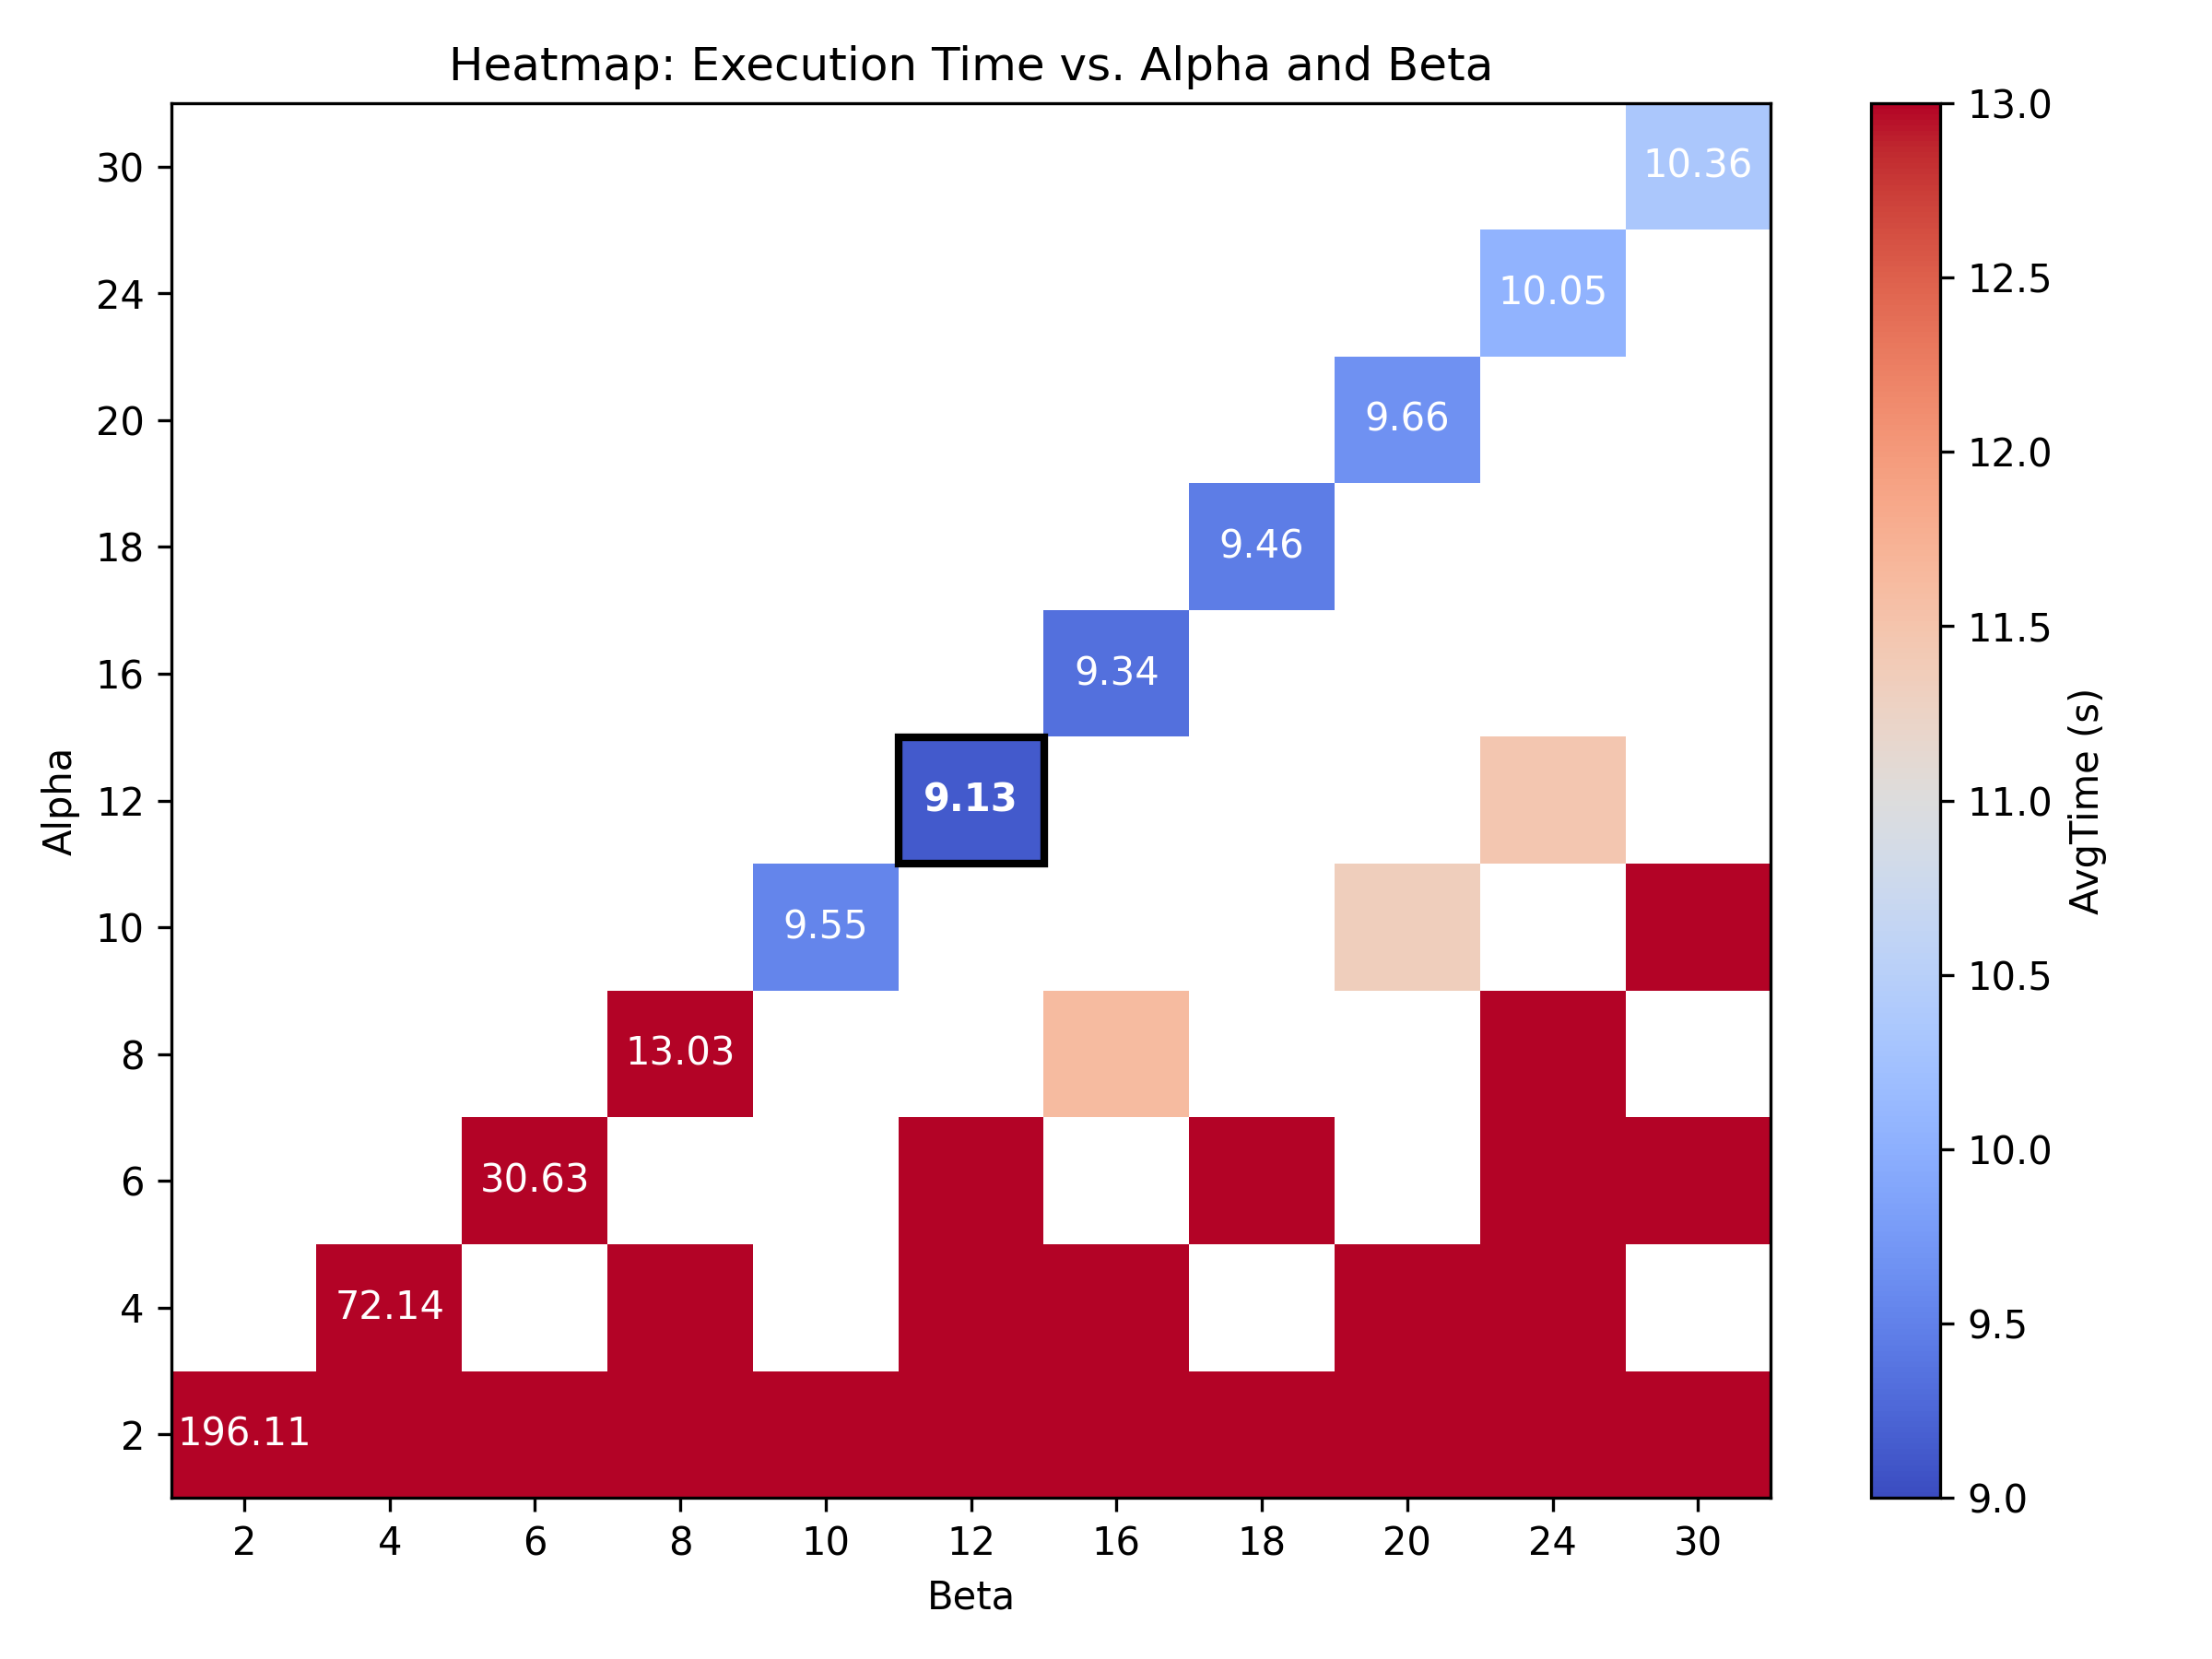
\includegraphics[width=\linewidth]{heatmap_without_priority.png}
        \caption{Without Priority}
        \label{fig:exp1_heatmap_a}
    \end{subfigure}\hfill
    \begin{subfigure}{0.5\linewidth}
        \centering
        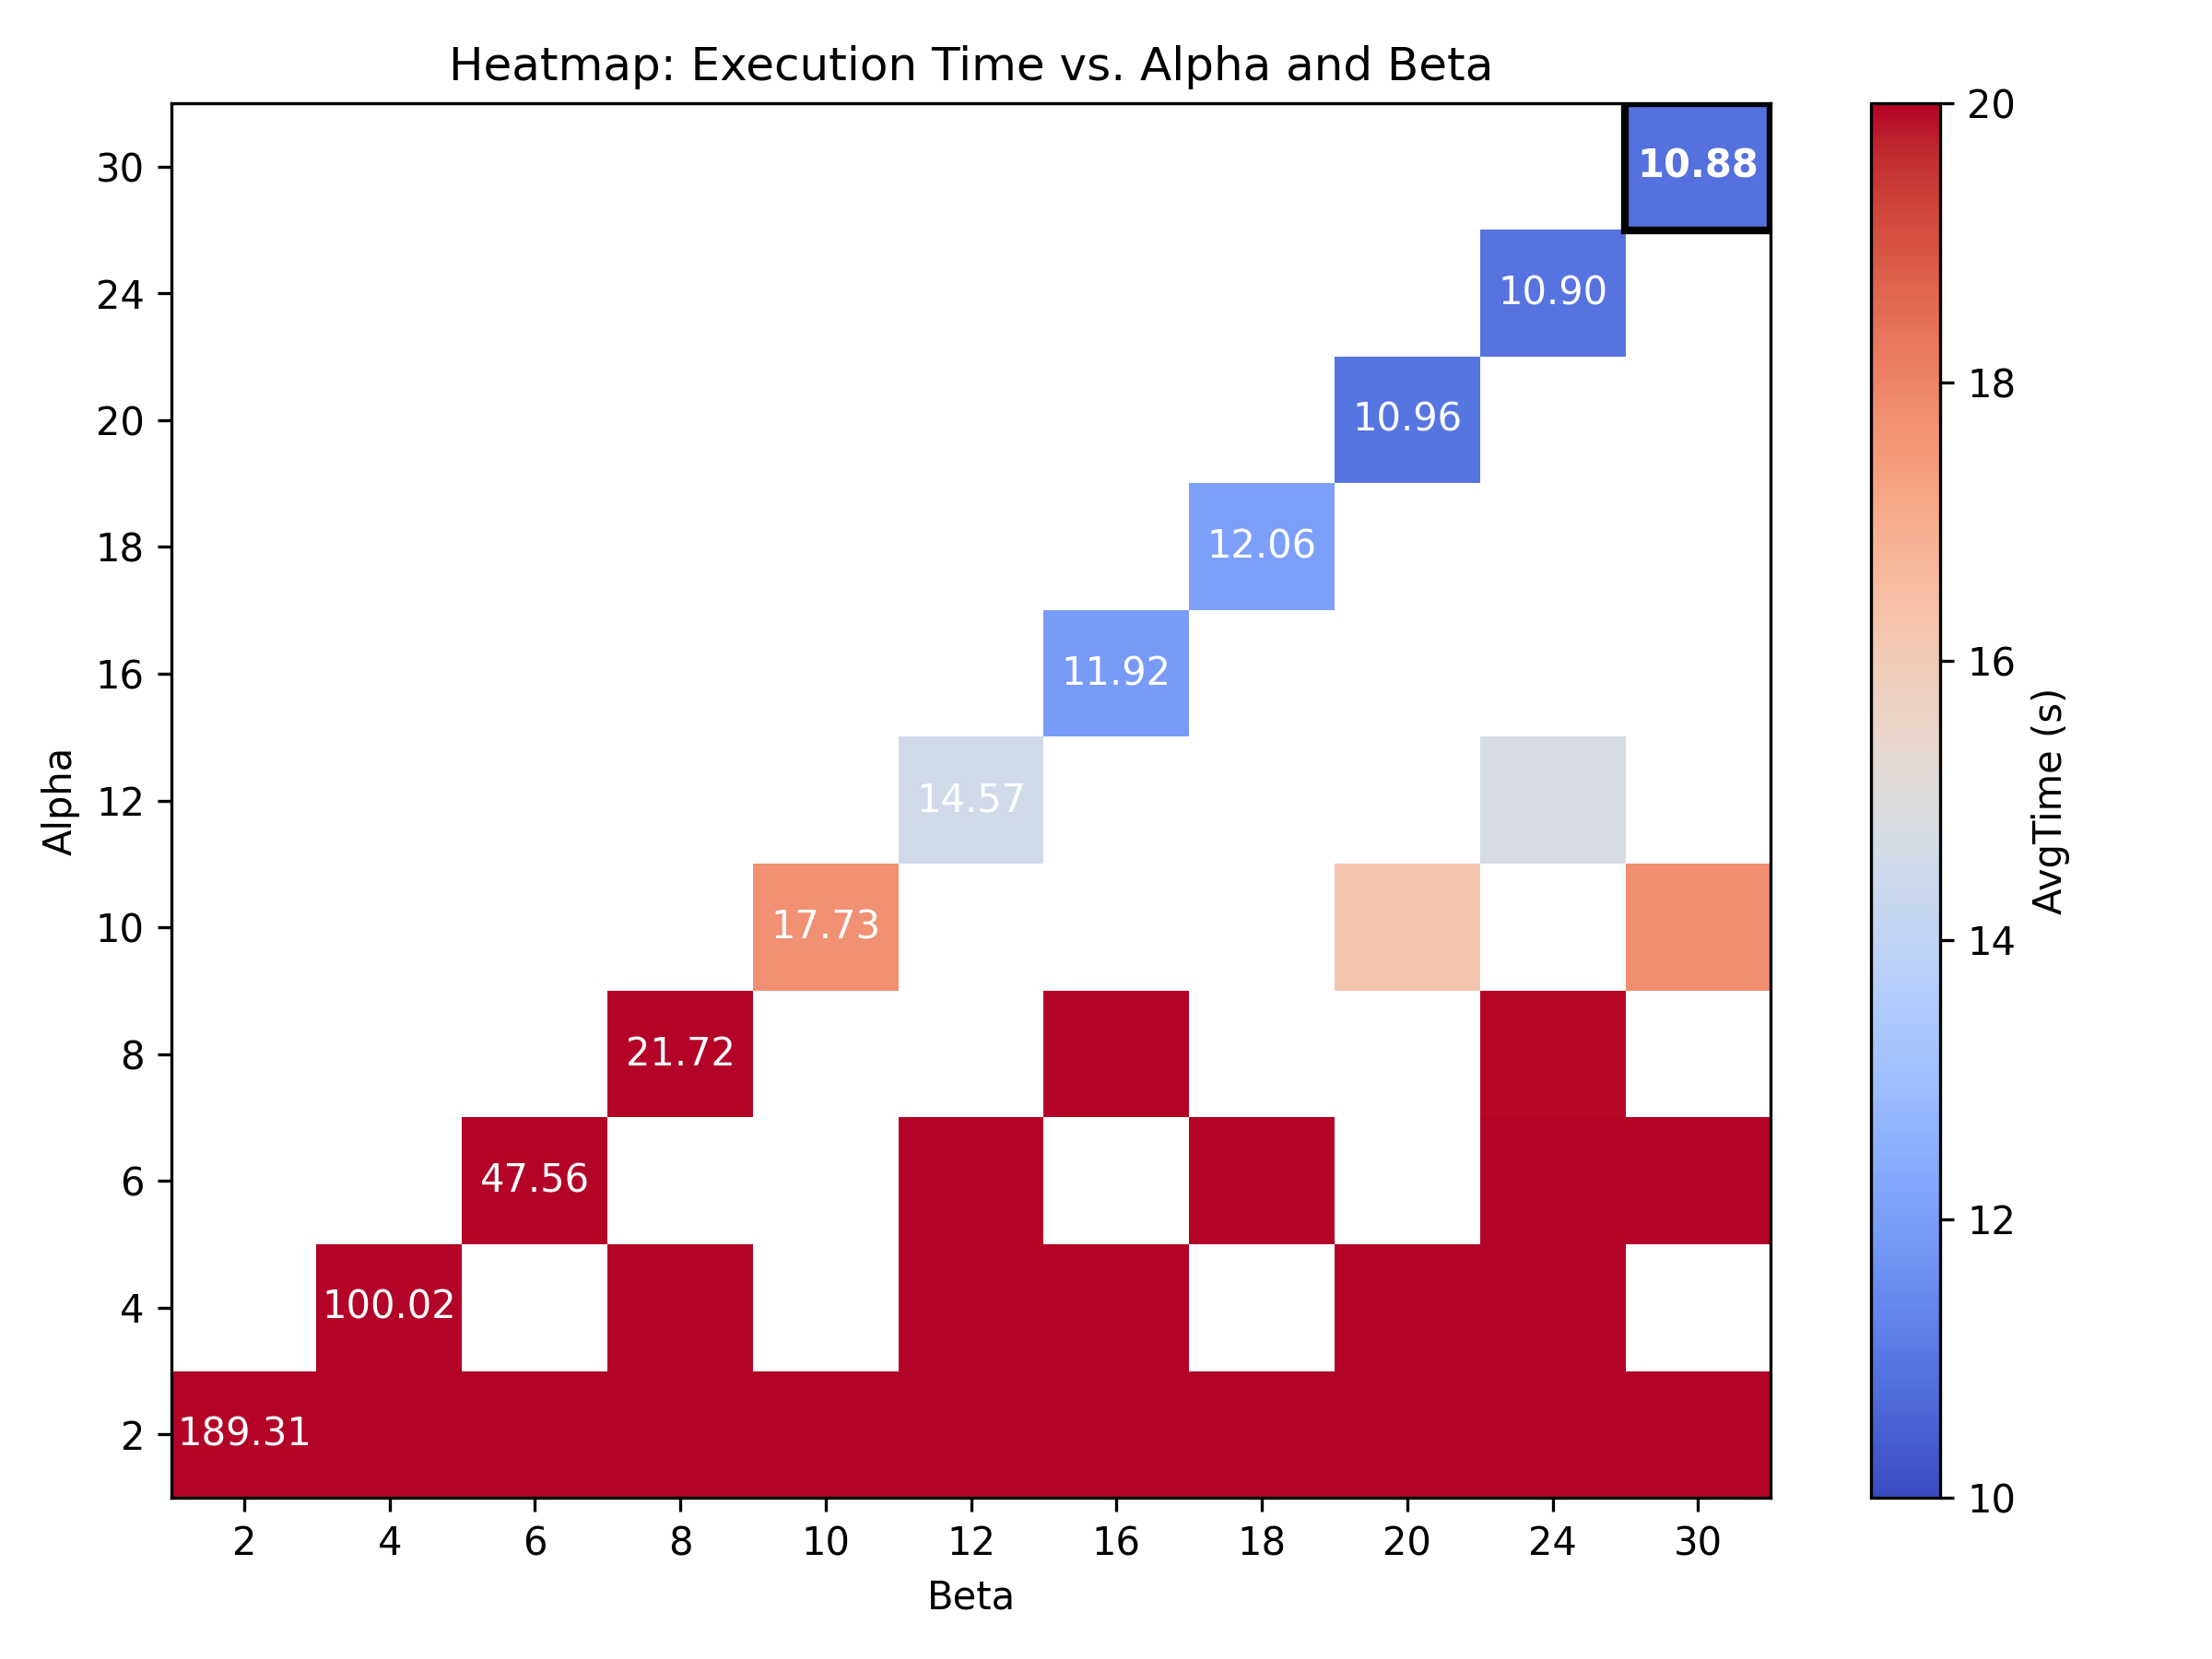
\includegraphics[width=\linewidth]{heatmap_with_priority.png}
        \caption{With Priority}
        \label{fig:exp1_heatmap_b}
    \end{subfigure}
    \caption{Heatmap views for the parameter sweep.}
    \label{fig:exp1_heatmap}
\end{figure}

\subsection{Parameter Tuning for Parallel QR Factorization}\label{exp:exp1}
\paragraph{(a) Heatmap Analysis:} 
In this experiment, an exhaustive sweep over the parameters $\alpha$ and $\beta$ (ranging from 2 to 32) was conducted on a fixed matrix size of $10800 \times 10800$ using 26 threads. The primary objective was to minimize execution time. Figure~\ref{fig:exp1_heatmap} presents heatmap visualizations for two cases: without priority scheduling and with priority scheduling. The results reveal that the optimal configuration occurs when $\alpha$ equals $\beta$, with $\alpha=\beta=12$ in the absence of priority scheduling and $\alpha=\beta=30$ under priority-based scheduling.
% \vspace{-0.7cm}


\paragraph{(b) Bar Graph Analysis:} Figure~\ref{fig:exp1_bar} illustrates the evolution of optimal $\alpha=\beta$ settings across various matrix sizes and thread counts (26, 52, and 104 threads), highlighting how computational load influences parameter tuning. The yellow highlighted band indicates the range in which the optimal parameter values consistently fall across different matrix sizes.
A key insight from the results is that, as the number of threads increases, the variability in the optimal $\alpha$–$\beta$ values diminishes. This convergence suggests that, under higher parallelism, finer granularity (i.e., lower $\alpha$ and $\beta$) is preferred to maximize workload distribution and minimize execution time.


\begin{figure}
    \centering
    % First bar plot (Without Priority) arranged vertically
    \begin{subfigure}{\linewidth}
        \centering
		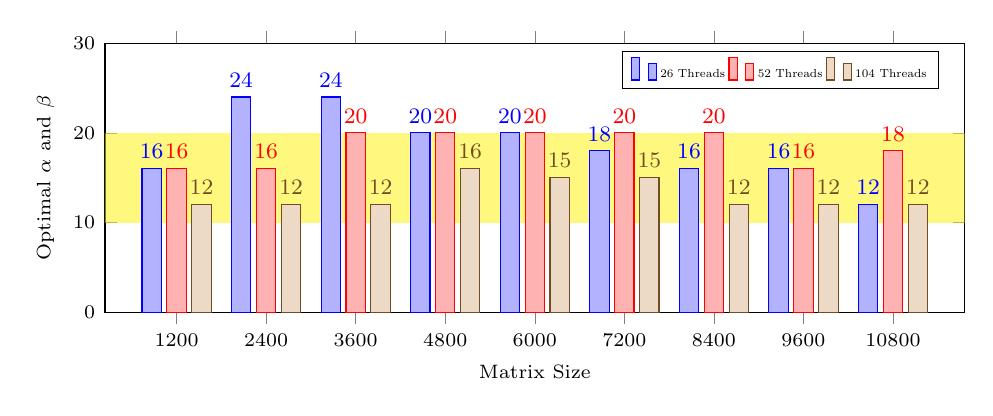
\begin{tikzpicture}
			\begin{axis}[
				ybar,
				bar width=7pt,
				symbolic x coords={300,600,1200,2400,3600,4800,6000,7200,8400,9600,10800,12000},
				xtick=data,
				xlabel={\scriptsize	 Matrix Size},
				ylabel={\scriptsize	 Optimal $\alpha$ and $\beta$},
				myBarStyle,
				tick label style={font=\scriptsize},
				label style={font=\scriptsize},
				legend style={font=\scriptsize	, nodes={scale=0.8, transform shape}, legend columns=-1, legend pos=north east},
				ymin=0, ymax=30,
				enlarge x limits=0.1,
				nodes near coords,
				every node near coord/.append style={font=\footnotesize}
				]
				\draw[draw=none,fill=yellow, fill opacity=0.5] 
				(axis cs:300,10) rectangle (axis cs:12000,20);
				
				\addplot coordinates {(1200,16) (2400,24) (3600,24) (4800,20) (6000,20) (7200,18) (8400,16) (9600,16) (10800,12)};
				\addplot coordinates {(1200,16) (2400,16) (3600,20) (4800,20) (6000,20) (7200,20) (8400,20) (9600,16) (10800,18)};
				\addplot coordinates {(1200,12) (2400,12) (3600,12) (4800,16) (6000,15) (7200,15) (8400,12) (9600,12) (10800,12)};
				\legend{26 Threads, 52 Threads, 104 Threads}
			\end{axis}
		\end{tikzpicture}
        \caption{Without Priority}
        \label{fig:exp1_bar_a}
    \end{subfigure}
    
    
    
    % Second bar plot (With Priority) arranged vertically
    \begin{subfigure}{\linewidth}
        \centering
		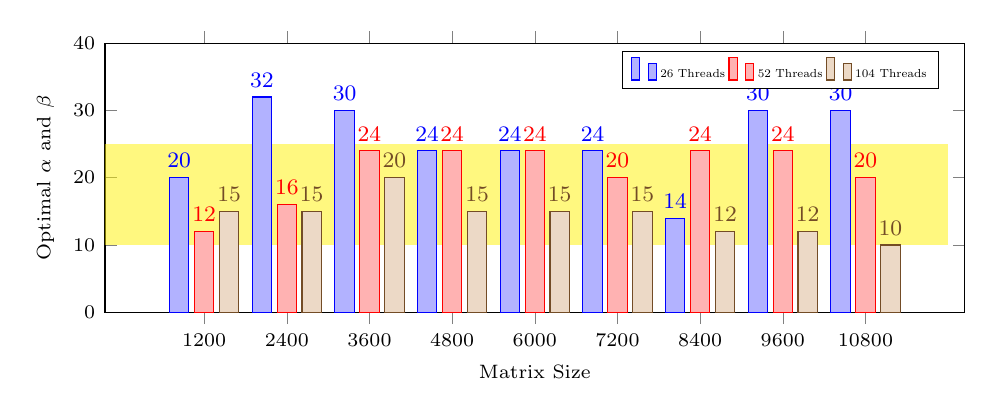
\begin{tikzpicture}
			\begin{axis}[
				ybar,
				bar width=7pt,
				symbolic x coords={300,600,1200,2400,3600,4800,6000,7200,8400,9600,10800,12000},
				xtick=data,
				xlabel={\scriptsize	 Matrix Size},
				ylabel={\scriptsize	 Optimal $\alpha$ and $\beta$},
				myBarStyle,
				tick label style={font=\scriptsize	},
				label style={font=\scriptsize	},
				legend style={font=\scriptsize	, nodes={scale=0.8, transform shape}, legend columns=-1, legend pos=north east},
				ymin=0, ymax=40,
				enlarge x limits=0.15,
				nodes near coords,
				every node near coord/.append style={font=\footnotesize}
				]
				\draw[draw=none,fill=yellow, fill opacity=0.5] 
				(axis cs:300,10) rectangle (axis cs:12000,25);
				
				\addplot coordinates {(1200,20) (2400,32) (3600,30) (4800,24) (6000,24) (7200,24) (8400,14) (9600,30) (10800,30)};
				\addplot coordinates {(1200,12) (2400,16) (3600,24) (4800,24) (6000,24) (7200,20) (8400,24) (9600,24) (10800,20)};
				\addplot coordinates {(1200,15) (2400,15) (3600,20) (4800,15) (6000,15) (7200,15) (8400,12) (9600,12) (10800,10)};
				\legend{26 Threads, 52 Threads, 104 Threads}
			\end{axis}
		\end{tikzpicture}
        \caption{With Priority}
        \label{fig:exp1_bar_b}
    \end{subfigure}
    
    \caption{Bar graphs of best configurations across different matrix sizes.}
    \label{fig:exp1_bar}
\end{figure}

\subsection{Scalability Analysis}\label{exp:exp2}
In this experiment, we assesses the scalability of our proposed algorithm on dense square matrices with dimensions ranging from $300 \times 300$ to $10800 \times 10800$. The optimal $\alpha$ and $\beta$ values determined in Experiment~\ref{exp:exp1} were employed consistently. To capture the impact of parallelism, tests were performed using 26 and 52 threads.

To assess the effectiveness of our approach, we compare three different methods: (i) a parallel DAG execution method that employs synchronization barriers and (ii) two variants of our proposed approach—one incorporating a priority-based scheduling mechanism and another without priority. This comparative analysis provides insights into the efficiency and scalability of the proposed methodology under varying computational loads.

Figure~\ref{fig:exp2_a} (26 threads) and Figure~\ref{fig:exp2_b} (52 threads) display the execution time trends as the matrix size increases. The results clearly demonstrate that both variants of our method (with and without priority scheduling) significantly outperform the barrier-based parallel DAG execution. However, the priority-free variant performs slightly better than priority-based due to the overhead introduced by priority queues. The additional overhead stems from the fact that priority queues reorder nodes according to their priority values and require more frequent data structure re-balancing.

\begin{figure}
    \centering
    \begin{subfigure}{0.5\linewidth}
        \centering
        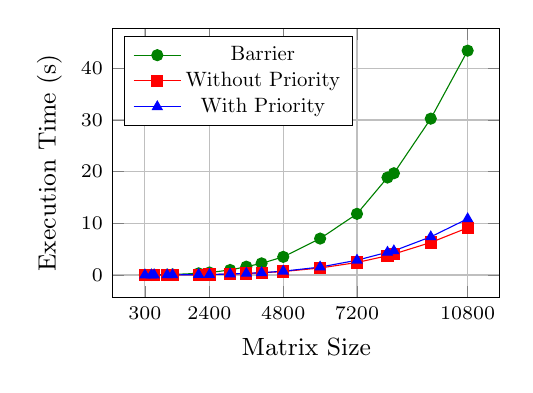
\begin{tikzpicture}
            \begin{axis}[
                xlabel={Matrix Size},
                ylabel={Execution Time (s)},
                xtick={300, 2400, 4800, 7200, 10800},
                xticklabels={300, 2400, 4800, 7200, 10800},
                ytick={0, 10, 20, 30, 40, 50},
                yticklabels={0, 10, 20, 30, 40, 50},
                scaled ticks=false,
                tick label style={/pgf/number format/fixed},
                myAxisStyle,
                legend style={nodes={scale=0.75, transform shape}},
                legend pos=north west
                ]
                \addplot[darkgreen, mark=*] coordinates {
                    (300,0.009) (512,0.019) (600,0.02467) (1024,0.072) (1200,0.095) (2048,0.31433) 
                    (2400,0.472) (3072,0.97033) (3600,1.60833) (4096,2.249) (4800,3.50733) 
                    (6000,7.049) (7200,11.83833) (8192,18.866) (8400,19.69433) (9600,30.26433) 
                    (10800,43.42867)
                };
                \addlegendentry{Barrier};
                
                \addplot[red, mark=square*] coordinates {
                    (300,0.002) (512,0.00433) (600,0.00533) (1024,0.01733) (1200,0.02067) (2048,0.06333) 
                    (2400,0.089) (3072,0.183) (3600,0.289) (4096,0.42933) (4800,0.66933) 
                    (6000,1.35233) (7200,2.41633) (8192,3.72667) (8400,4.063) 
                    (9600,6.28833) (10800,9.13267)
                };
                \addlegendentry{Without Priority};
                
                \addplot[blue, mark=triangle*] coordinates {
                    (300,0.002) (512,0.005) (600,0.00567) (1024,0.01667) (1200,0.021) (2048,0.06133) 
                    (2400,0.08733) (3072,0.18533) (3600,0.30633) (4096,0.44233) (4800,0.73167) 
                    (6000,1.53133) (7200,2.85767) (8192,4.401) (8400,4.67167) 
                    (9600,7.387) (10800,10.87967)
                };
                \addlegendentry{With Priority};
            \end{axis}
        \end{tikzpicture}
        \caption{Exec. Time vs Matrix Size (26 Threads)}
        \label{fig:exp2_a}
    \end{subfigure}\hfill
    \begin{subfigure}{0.5\linewidth}
        \centering
        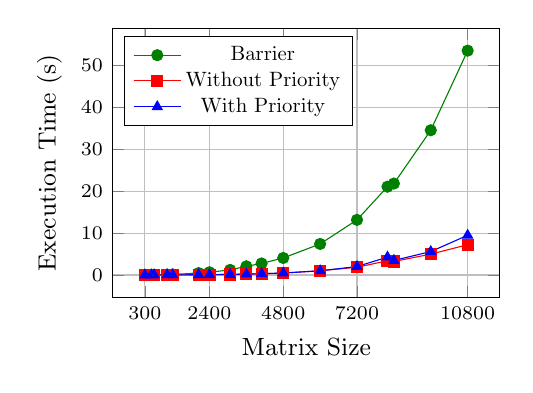
\begin{tikzpicture}
            \begin{axis}[
                xlabel={Matrix Size},
                ylabel={Execution Time (s)},
                xtick={300, 2400, 4800, 7200, 10800},
                xticklabels={300, 2400, 4800, 7200, 10800},
                ytick={0, 10, 20, 30, 40, 50},
                yticklabels={0, 10, 20, 30, 40, 50},
                scaled ticks=false,
                tick label style={/pgf/number format/fixed},
                myAxisStyle,
                legend style={nodes={scale=0.75, transform shape}},
                legend pos=north west
                ]
                \addplot[darkgreen, mark=*] coordinates {
                    (300,0.01367) (512,0.02867) (600,0.038) (1024,0.08867) (1200,0.12633) 
                    (2048,0.44633) (2400,0.646) (3072,1.20967) (3600,2.06267) 
                    (4096,2.74733) (4800,4.058) (6000,7.4) (7200,13.15033) 
                    (8192,21.07267) (8400,21.81733) (9600,34.544) (10800,53.54133)
                };
                \addlegendentry{Barrier};
                
                \addplot[red, mark=square*] coordinates {
                    (300,0.00267) (512,0.00567) (600,0.00667) (1024,0.01567) (1200,0.01933) 
                    (2048,0.04767) (2400,0.069) (3072,0.13033) (3600,0.195) (4096,0.28833) 
                    (4800,0.454) (6000,1.00233) (7200,1.838) (8192,3.39833) 
                    (8400,3.21767) (9600,4.96967) (10800,7.22533)
                };
                \addlegendentry{Without Priority};
                
                \addplot[blue, mark=triangle*] coordinates {
                    (300,0.00333) (512,0.007) (600,0.00767) (1024,0.01733) (1200,0.019) 
                    (2048,0.04967) (2400,0.066) (3072,0.12633) (3600,0.191) (4096,0.30833) 
                    (4800,0.45567) (6000,0.99867) (7200,2.00967) (8192,4.25967) 
                    (8400,3.464) (9600,5.58033) (10800,9.47167)
                };
                \addlegendentry{With Priority};
            \end{axis}
        \end{tikzpicture}
        \caption{Exec. Time vs Matrix Size (52 Threads)}
        \label{fig:exp2_b}
    \end{subfigure}
    \caption{Scalability comparison of the proposed algorithm for different matrix sizes.}
    \label{fig:exp2}
\end{figure}

\begin{figure}
    \centering
    \begin{minipage}{0.5\linewidth}
        \centering
        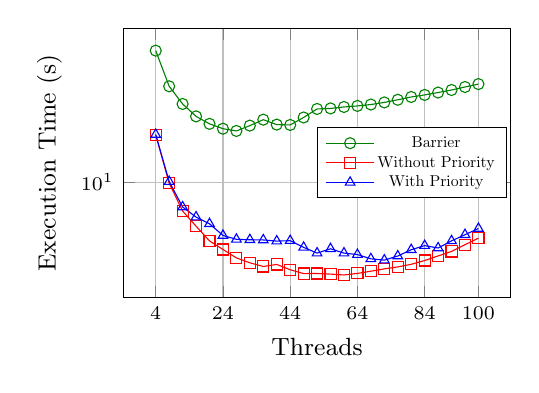
\begin{tikzpicture}
            \begin{axis}[
                xlabel={Threads},
                ylabel={Execution Time (s)},
                myAxisStyle,
                ymode=log,
                log basis y=10,
                xtick={4, 24, 44, 64, 84, 100},
                ytick={10, 100, 1000, 10000, 100000},
                legend style={at={(axis description cs:0.5,0.5)}, anchor=west, nodes={scale=0.57, transform shape}}
                ]
                \addplot[darkgreen, mark=o] coordinates {
                    (4,60.32933) (8,37.08767) (12,29.13767) (16,24.59833)
                    (20,22.211) (24,20.787) (28,20.160) (32,21.67867)
                    (36,23.511) (40,21.980) (44,21.87833) (48,24.22767)
                    (52,27.220) (56,27.414) (60,27.967) (64,28.367)
                    (68,28.91533) (72,29.754) (76,30.85733) (80,32.056)
                    (84,32.97067) (88,34.05467) (92,35.255) (96,36.73167)
                    (100,38.23033)
                };
                \addlegendentry{Barrier};
                
                \addplot[red, mark=square] coordinates {
                    (4,19.068) (8,9.88267) (12,6.753) (16,5.495)
                    (20,4.492) (24,3.996) (28,3.563) (32,3.33167)
                    (36,3.169) (40,3.258) (44,3.030) (48,2.87633)
                    (52,2.87967) (56,2.85433) (60,2.82233) (64,2.883)
                    (68,2.971) (72,3.06733) (76,3.15033) (80,3.26467)
                    (84,3.438) (88,3.65933) (92,3.891) (96,4.26467)
                    (100,4.668)
                };
                \addlegendentry{Without Priority};
                
                \addplot[blue, mark=triangle] coordinates {
                    (4,19.20933) (8,10.104) (12,7.13767) (16,6.22233)
                    (20,5.67667) (24,4.84067) (28,4.59033) (32,4.56433)
                    (36,4.55167) (40,4.48067) (44,4.507) (48,4.11267)
                    (52,3.804) (56,4.03433) (60,3.80433) (64,3.72833)
                    (68,3.518) (72,3.45633) (76,3.65533) (80,3.98367)
                    (84,4.212) (88,4.07933) (92,4.493) (96,4.891)
                    (100,5.32067)
                };
                \addlegendentry{With Priority};
            \end{axis}
        \end{tikzpicture}
        \caption{Throughput Evaluation}
        \label{fig:fig4}
    \end{minipage}\hfill
    \begin{minipage}{0.49\linewidth}
        \centering
        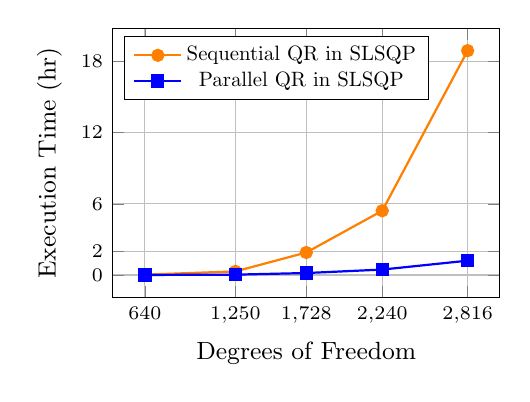
\begin{tikzpicture}
            \begin{axis}[
                xlabel={Degrees of Freedom},
                ylabel={Execution Time (hr)},
                myAxisStyle,
                legend style={nodes={scale=0.75, transform shape}},
                xtick={640,1250,1728,2240,2816},
                ytick={0,2,6,12,18},
                legend pos=north west
                ]
                \addplot[orange, mark=*, thick] coordinates {
                    (640,0.02908)
                    (1250,0.3004)
                    (1728,1.89514)
                    (2240,5.415)
                    (2816,18.91215)
                };
                \addlegendentry{Sequential QR in SLSQP};
                
                \addplot[blue, mark=square*, thick] coordinates {
                    (640,0.001454)
                    (1250,0.02879)
                    (1728,0.16458)
                    (2240,0.456)
                    (2816,1.20716)
                };
                \addlegendentry{Parallel QR in SLSQP};
            \end{axis}
        \end{tikzpicture}
        \caption{SLSQP  Performance}
        \label{fig:fig5}
    \end{minipage}
\end{figure}

\subsection{Throughput Evaluation} \label{exp:exp3}
% In this experiment, we evaluate the throughput of multiple algorithms by increasing the number of threads(in the multiples of 4) for a fixed matrix size of $8192 \times 8192$. The optimal $\alpha$ and $\beta$ values identified in Experiment~1 are employed for this study. Three approaches are compared: the parallel DAG execution method using synchronization barriers, and two variants of our proposed method—one incorporating a priority-based mechanism and one without.
In this experiment, we evaluate the throughput of various algorithms by incrementally increasing the number of threads (in multiples of 4) for a fixed matrix size of $8192 \times 8192$, while using the optimal $\alpha$ and $\beta$ values from Experiment~\ref{exp:exp1}. Figure~\ref{fig:fig4} plots the execution time (on a logarithmic scale) against thread count for three methods: barrier-based, without priority, and with priority scheduling.

The results align with the previous experiment, confirming that our proposed method (with and without priority) outperforms the parallel DAG execution with barriers. However, the priority-based variant is slightly less efficient due to its additional overhead.

% Experiment 3 and 4 arranged side by side as Fig.4 and Fig.5 respectively.


\subsection{Impact of Parallel QR Factorization in SLSQP} \label{exp:exp4}

In this experiment, we examine the influence of integrating our proposed parallel QR approach into the SLSQP framework within the NLOPT library. Our focus is on large-scale boundary value problems involving implicit constitutive relations under both elastic and inelastic responses.\cite{ananthapadmanabhan2023multi}.

To assess performance, we compare a baseline SLSQP implementation equip-ped with sequential QR factorization against an SLSQP version that leverages our parallel QR factorization. We evaluated these approaches over a range of problem sizes defined by degrees of freedom (DOF) equal to 640, 1250, 1728, 2240, and 2816. Here, the term "degrees of freedom" denotes the total number of unknowns, such as nodal displacements, stresses, or auxiliary state variables, emerging from the discretizations of the governing partial differential equations and boundary conditions. Consequently, an increase in DOF results in a proportional increase in the dimension of the system matrix factorized by SLSQP.

Figure~\ref{fig:fig5} shows the execution times (in hours) corresponding to each DOF level for both sequential and parallel QR implementations. Notably, when the DOF reaches 2816, the parallel QR variant completes its tasks in approximately 1.21~hours, whereas the sequential counterpart requires nearly 18.91~hours. This substantial improvement in computational efficiency becomes increasingly pronounced as the DOF grows, reflecting the strong scalability of the parallel approach.
